\documentclass[12pt]{article}
\usepackage[utf8]{inputenc}
\usepackage{a4,amsmath,amsfonts,amsthm,latexsym,amssymb,graphicx}
\usepackage{tikz}
\usepackage{tikz-cd}
\usepackage{pgf}

\begin{document}

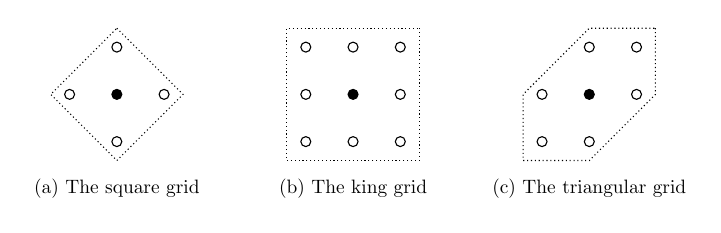
\begin{tikzpicture}[scale=0.6]
		% square grid neighborhood r=1
		\draw[fill=black] (0,0) circle(3pt);
		\draw (-1,0) circle(3pt);
		\draw (0,-1) circle(3pt);
		\draw (1,0) circle(3pt);
		\draw (0,1) circle(3pt);
		
		\draw[densely dotted] (0,1.4) -- (1.4,0) -- (0,-1.4) -- (-1.4,0) -- (0,1.4);
		\node[scale=0.7] at (0,-2) {(a) The square grid};
		
		% king grid neighborhood r=1
		\draw[fill=black] (5,0) circle(3pt);
		\draw (4,0) circle(3pt);
		\draw (5,-1) circle(3pt);
		\draw (6,0) circle(3pt);
		\draw (5,1) circle(3pt);	
		\draw (6,1) circle(3pt);	
		\draw (6,-1) circle(3pt);
		\draw (4,1) circle(3pt);
		\draw (4,-1) circle(3pt);
		
		\draw[densely dotted] (6.4,1.4) -- (6.4,-1.4) -- (3.6,-1.4) -- (3.6,1.4) -- (6.4,1.4);
		\node[scale=0.7] at (5,-2) {(b) The king grid};
		
		% triangular grid neighborhood r=1		
		\draw[fill=black] (10,0) circle(3pt);
		\draw (9,0) circle(3pt);
		\draw (10,-1) circle(3pt);
		\draw (11,0) circle(3pt);
		\draw (10,1) circle(3pt);	
		\draw (11,1) circle(3pt);	
		\draw (9,-1) circle(3pt);
		
		\draw[densely dotted] (11.4,1.4) -- (11.4,0) -- (10,-1.4) -- (8.6,-1.4) -- (8.6,0) -- (10,1.4) -- (11.4,1.4);
		\node[scale=0.7] at (10,-2) {(c) The triangular grid};
	\end{tikzpicture}

\end{document}